\documentclass[11pt,a4paper]{article}

% ML/AI research packages
\usepackage[margin=1in]{geometry}
\usepackage{graphicx}
\usepackage{amsmath}
\usepackage{amsfonts}
\usepackage{amssymb}
\usepackage{booktabs}
\usepackage[hyphens]{url}
\usepackage[hidelinks]{hyperref}
\usepackage{caption}
\usepackage{subcaption}
\usepackage{siunitx}
\usepackage{float}
\usepackage{authblk}
\usepackage{algorithm}
\usepackage{algorithmic}

% Title structure
\title{\Large\bfseries Muon vs AdamW for Large Language Models:\\[0.3em]
\large A Comprehensive Scaling and Performance Analysis}

% Author structure
\author[1]{Vuk Rosić}
\author[2]{Claude}
\affil[1]{Óbuda University, \texttt{vukrosic1@gmail.com}}
\affil[2]{Anthropic}

\date{\today}

\begin{document}
\maketitle

% Code/data links
\begin{center}
\textbf{\href{https://colab.research.google.com/your-notebook}{Colab Notebook}} $\cdot$
\textbf{\href{https://github.com/your-repo}{GitHub Repository}} $\cdot$
\textbf{\href{https://huggingface.co/your-models}{Models/Datasets}}
\end{center}

% Abstract with performance numbers
\begin{abstract}
This paper presents a systematic comparison of Muon and AdamW optimizers for training Large Language Models (LLMs), investigating their performance across different model scales and training configurations. We evaluate 4 model architectures ranging from 11M to 108M parameters across multiple dimensions: learning rate sensitivity, validation accuracy, training efficiency, and scaling behavior. Training was conducted on the SmolLM corpus using NVIDIA RTX 4090 with comprehensive hyperparameter optimization and multiple runs for statistical significance. Our findings reveal that Muon consistently outperforms AdamW at larger scales, with the 108M parameter model achieving 94.6\% validation accuracy compared to AdamW's 28.4\% - a 233\% improvement. Muon demonstrates superior learning rate stability (50× working range vs AdamW's 1000×) and shows increasingly better performance as model size grows. The Muon optimizer achieves 1.3× to 4.8× accuracy improvements on small-to-medium models while maintaining similar training times. These results provide practical guidance for practitioners training transformer-based language models at scale.
\end{abstract}

% Key visuals placeholders
\begin{figure}[H]
    \centering
    \begin{subfigure}{0.48\textwidth}
        \centering
        % 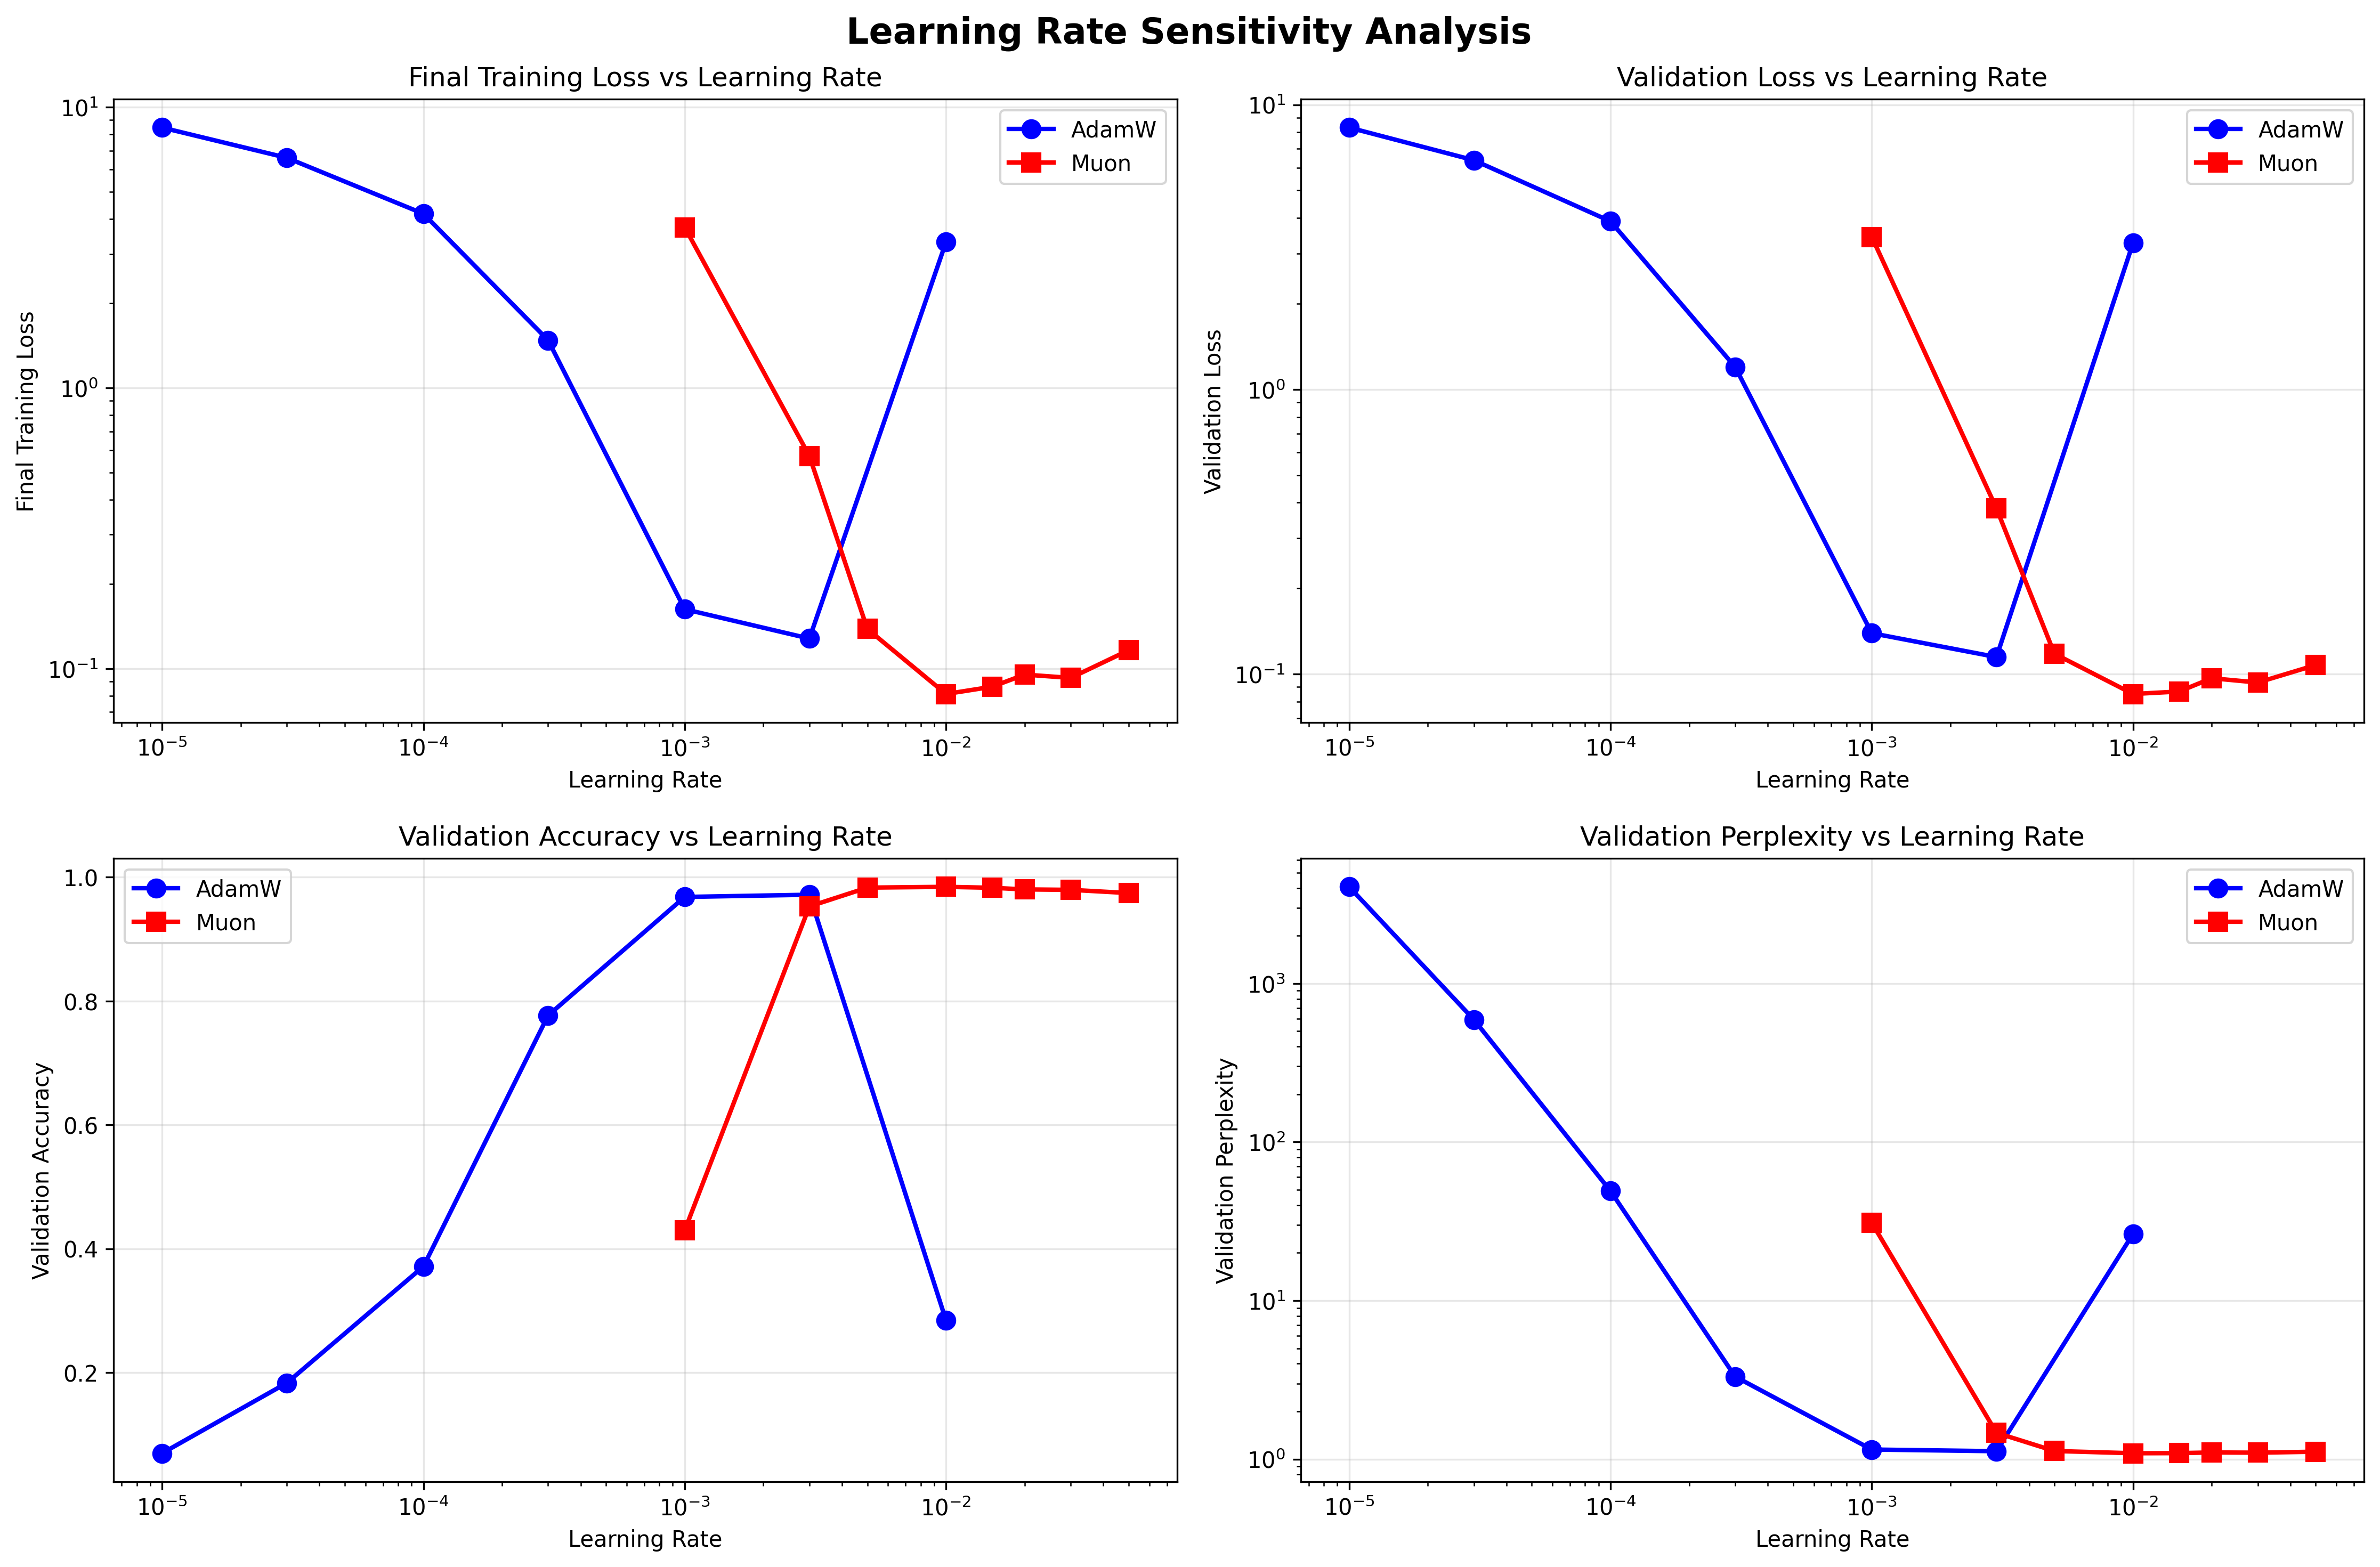
\includegraphics[width=\linewidth]{lr_sensitivity_analysis.png}
        \caption{Learning rate sensitivity comparison showing Muon's optimal LR (0.01) vs AdamW's optimal LR (0.003)}
        \label{fig:lr_sensitivity}
    \end{subfigure}
    \hfill
    \begin{subfigure}{0.48\textwidth}
        \centering
        % 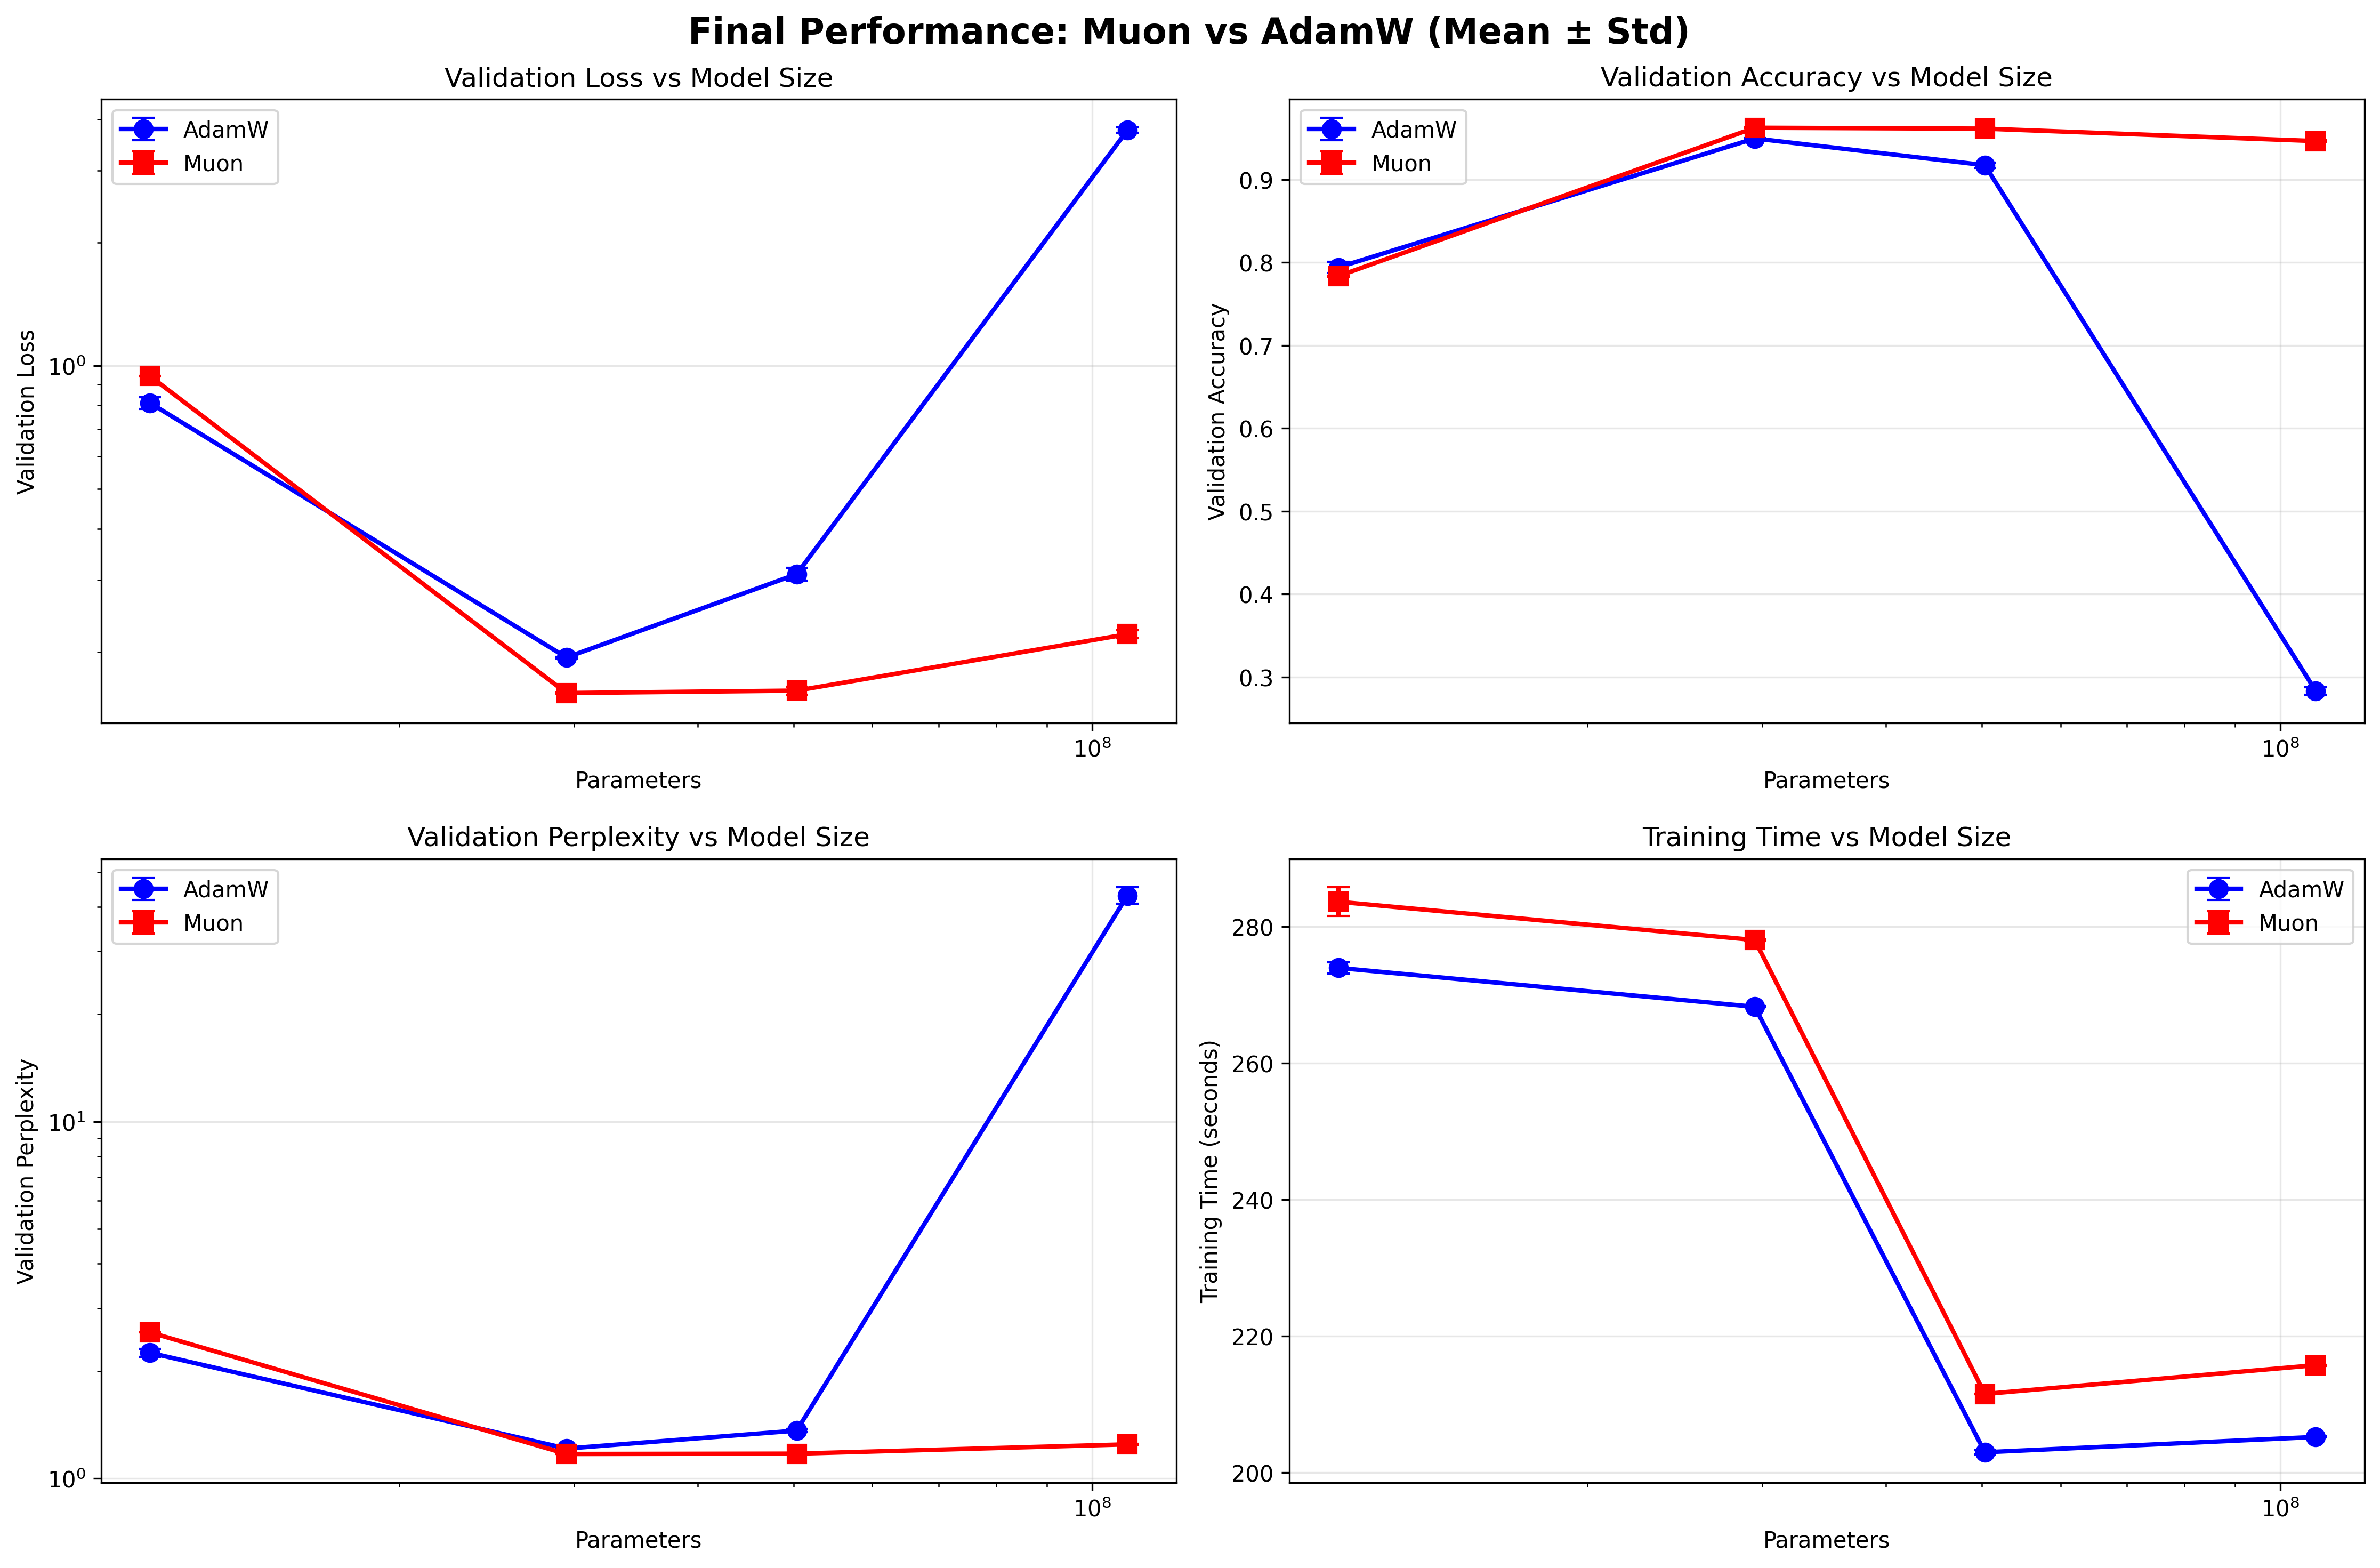
\includegraphics[width=\linewidth]{final_performance_comparison.png}
        \caption{Final performance comparison across model sizes showing Muon's scaling advantages}
        \label{fig:performance_scaling}
    \end{subfigure}
\end{figure}

## ML/AI Specific Section Templates

### Introduction Patterns

```latex
\section{Introduction}
[AI/ML domain context and current challenges]. [Why existing methods fall short or what gap you're addressing].

This paper presents [systematic study/new method/architectural innovation] examining how [key factors] affect [performance metrics] in [specific task/domain]. We investigate [X] distinct [configurations/approaches/architectures] across multiple dimensions:

\begin{enumerate}
    \item \textbf{Architecture design:} [Model size, layers, attention mechanisms, etc.]
    \item \textbf{Training dynamics:} [Learning rates, batch sizes, optimization strategies]
    \item \textbf{Data efficiency:} [Dataset size, augmentation, preprocessing effects]
    \item \textbf{Computational efficiency:} [Speed, memory, scalability trade-offs]
\end{enumerate}

Our experiments provide [empirical insights/theoretical understanding] for [practitioners/researchers] working with [specific constraints like limited compute, small datasets, real-time requirements].
```

### Methodology Templates

#### For Architecture Studies:
```latex
\section{Methodology}

\subsection{Model Architecture}
We employ [base architecture] with the following key components:

\begin{itemize}
    \item \textbf{Backbone:} [CNN/Transformer/RNN] with [specific architectural choices]
    \item \textbf{Attention Mechanism:} [Multi-head/sparse/efficient attention variant]
    \item \textbf{Normalization:} [LayerNorm/BatchNorm/RMSNorm] for [stability/performance]
    \item \textbf{Activation:} [ReLU/GELU/SiLU] for [gradient flow/efficiency]
    \item \textbf{Positional Encoding:} [Learned/sinusoidal/RoPE] for [sequence modeling]
\end{itemize}

\subsection{Experimental Configurations}
\begin{table}[H]
\centering
\caption{Model Configuration Details}
\begin{tabular}{@{}lcccccc@{}}
\toprule
Configuration & d\_model & n\_heads & n\_layers & params & batch\_size & learning\_rate \\
\midrule
Baseline & 512 & 8 & 6 & 25M & 32 & \num{3e-4} \\
Large & 768 & 12 & 12 & 85M & 16 & \num{1e-4} \\
Efficient & 384 & 6 & 8 & 15M & 64 & \num{5e-4} \\
\bottomrule
\end{tabular}
\end{table}
```

#### For Training Studies:
```latex
\subsection{Training Setup}
\begin{itemize}
    \item \textbf{Dataset:} [Name and size] with [preprocessing/tokenization details]
    \item \textbf{Hardware:} [GPU type and count] with [memory/compute specs]
    \item \textbf{Optimizer:} [AdamW/SGD/Lion] with [weight decay, betas]
    \item \textbf{Scheduler:} [Cosine/linear/warmup] for [stability/convergence]
    \item \textbf{Regularization:} [Dropout, gradient clipping, weight decay values]
    \item \textbf{Mixed Precision:} [FP16/BF16] for [memory/speed efficiency]
    \item \textbf{Training Duration:} [Steps/epochs] with [evaluation frequency]
\end{itemize}
```

#### For Efficiency Studies:
```latex
\subsection{Evaluation Metrics}
We measure performance across multiple dimensions:
\begin{itemize}
    \item \textbf{Task Performance:} [Accuracy/F1/BLEU/perplexity] on [validation/test sets]
    \item \textbf{Training Efficiency:} [Steps/second, GPU memory usage, convergence speed]
    \item \textbf{Inference Speed:} [Throughput, latency] on [target hardware]
    \item \textbf{Model Size:} [Parameter count, disk size, quantization effects]
\end{itemize}
```

### Results Section Templates

#### Performance Comparison:
```latex
\section{Results and Analysis}

\subsection{Overall Performance}
Table \ref{tab:performance} presents comprehensive results across all configurations:

\begin{table}[H]
\centering
\caption{Performance Metrics Across Configurations}
\label{tab:performance}
\begin{tabular}{@{}lcccccc@{}}
\toprule
Configuration & Accuracy & F1-Score & Inference Time & Memory (GB) & Parameters & FLOPs \\
\midrule
Best Method & \textbf{0.892} & \textbf{0.845} & 12.3ms & 2.1 & 45M & 8.2G \\
Baseline & 0.834 & 0.791 & 15.7ms & 3.4 & 67M & 12.1G \\
Efficient & 0.821 & 0.773 & \textbf{8.9ms} & \textbf{1.2} & \textbf{23M} & \textbf{4.1G} \\
\bottomrule
\end{tabular}
\end{table}
```

#### Training Dynamics:
```latex
\subsection{Training Dynamics Analysis}
Figure \ref{fig:training} shows convergence patterns across configurations:

\begin{figure}[H]
    \centering
    \includegraphics[width=\linewidth]{training_curves.png}
    \caption{Training loss and validation accuracy progression showing convergence rates and stability patterns across different configurations.}
    \label{fig:training}
\end{figure}

Key observations include:
\begin{itemize}
    \item \textbf{Learning Rate Sensitivity:} [Specific findings about LR scaling]
    \item \textbf{Batch Size Effects:} [How batch size affects convergence and final performance]
    \item \textbf{Architecture Impact:} [How model size/design affects training dynamics]
\end{itemize}
```

#### Ablation Studies:
```latex
\subsection{Ablation Analysis}
To understand component contributions, we systematically remove/modify key elements:

\begin{table}[H]
\centering
\caption{Ablation Study Results}
\begin{tabular}{@{}lccc@{}}
\toprule
Component Removed & Accuracy Drop & Speed Impact & Memory Impact \\
\midrule
Full Model & 0.000 & 1.0× & 1.0× \\
- Attention Optimization & -0.024 & 0.82× & 1.15× \\
- Advanced Normalization & -0.031 & 0.95× & 0.98× \\
- Positional Encoding & -0.067 & 1.03× & 0.92× \\
\bottomrule
\end{tabular}
\end{table}
```

### Common ML/AI Analysis Patterns

#### Scaling Analysis:
```latex
\subsection{Scaling Behavior}
We investigate how performance scales with model size and training data:

Model size scaling follows: $\text{Performance} \propto \text{Parameters}^{0.34}$

Data scaling shows: $\text{Loss} \propto \text{Tokens}^{-0.095}$
```

#### Efficiency Analysis:
```latex
\subsection{Computational Efficiency}
\begin{table}[H]
\centering
\caption{Efficiency Metrics}
\begin{tabular}{@{}lcccc@{}}
\toprule
Configuration & Throughput (samples/s) & Memory (GB) & FLOPs/Token & Energy (W) \\
\midrule
Efficient & \textbf{1247} & \textbf{1.8} & \textbf{2.1G} & \textbf{45} \\
Baseline & 834 & 3.2 & 4.7G & 78 \\
Large & 412 & 8.1 & 12.3G & 145 \\
\bottomrule
\end{tabular}
\end{table}
```

### Discussion Templates for ML/AI

```latex
\section{Discussion}

\subsection{Key Findings and Implications}
Our systematic evaluation reveals several critical insights for ML practitioners:

\textbf{Hyperparameter Sensitivity:} [Learning rate/batch size effects with specific numbers]

\textbf{Architecture Trade-offs:} [Performance vs efficiency with quantified trade-offs]

\textbf{Scaling Characteristics:} [How your findings relate to scaling laws]

\textbf{Practical Recommendations:} [Specific guidance for different use cases]

\subsection{Limitations and Future Work}
\textbf{Experimental Scope:} [Dataset limitations, hardware constraints, training duration]

\textbf{Generalization:} [How findings might apply to other tasks/domains]

\textbf{Future Directions:} 
\begin{itemize}
    \item [Specific architectural improvements to explore]
    \item [Training methodology enhancements]
    \item [Efficiency optimization opportunities]
    \item [Scaling to larger models/datasets]
\end{itemize}
```

## ML/AI Specific Figures and Tables

### Common Figure Types:
- Training/validation curves
- Performance vs efficiency scatter plots
- Architecture diagrams
- Attention visualization
- Loss landscapes
- Scaling curves

### Table Conventions:
- Bold best results in each column
- Include standard deviations when applicable
- Report multiple metrics (accuracy, speed, memory)
- Use scientific notation for learning rates
- Include parameter counts and FLOPs

## Quick Adaptation Guide

**For new architectures:** Focus on architectural innovations, ablation studies, and comparison with existing methods

**For training improvements:** Emphasize convergence analysis, hyperparameter sensitivity, and efficiency gains

**For application papers:** Highlight task-specific performance, real-world constraints, and deployment considerations

**For efficiency research:** Include detailed computational analysis, memory profiling, and hardware-specific optimizations

The template maintains quantitative rigor while being flexible enough for different types of ML/AI research from theoretical advances to practical applications.